%dilated polytope 3x where ldsegments disappear

\begin{figure}[ht!]
    \centering
    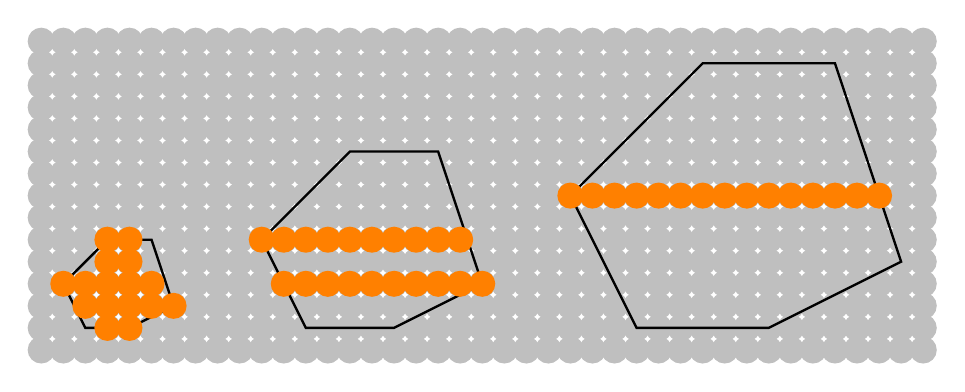
\begin{tikzpicture}[thin, scale=0.28]\vspace{0.5cm}
        \foreach \x in {-4,...,36} {
            \foreach \y in {-1,...,13} {
                \node at (\x,\y) [circle, draw=lightgray, fill= lightgray, minimum width=1.5pt] {};   
            }
        }
    
    %Outline of polytopes 1P, 2P, 3P
    \draw[line width=0.3mm, black] (-2,0) -- (-3,2) --(-1,4) --(1,4) -- (2,1)-- (0,0) -- cycle;
    \draw[line width=0.3mm, black](8,0) -- (6,4) -- (10,8) -- (14,8) -- (16,2) -- (12,0) -- cycle;
    \draw[line width=0.3mm, black] (23,0) -- (20,6) -- (26,12) -- (32,12) -- (35,3) -- (29,0) -- cycle;

    
    %Lattice Diameters in P
    %full segments L \cap P
    % \draw[line width=0.3mm, orange] (-3,2) -- (1.66,2);
    % \draw[line width=0.3mm, orange] (-2.5,1) -- (2,1);
    
    %ends at last lattice point
    \draw[line width=0.3mm, orange] (-3,2) -- (1,2);
    \draw[line width=0.3mm, orange] (-2,1) -- (2,1);
    
    %same for both
    \draw[line width=0.3mm, orange] (-1,0) -- (-1,4);
    \draw[line width=0.3mm, orange] (0,0) -- (0,4);

     \foreach \x in {-2, ..., 2} {
    \node at (\x,1) [circle, fill=orange, minimum width=3pt] {};
        }
    \foreach \x in {-3, ..., 1} {
    \node at (\x,2) [circle, fill=orange, minimum width=3pt] {};
        }
    \foreach \y in {0, ..., 4} {
    \node at (-1,\y) [circle, fill=orange, minimum width=3pt] {};
    \node at (0,\y) [circle, fill=orange, minimum width=3pt] {};
        }

        
    %Lattice Diameters in 2P
    %\draw[line width=0.3mm, orange] (6,4) -- (15.32,4);
    \draw[line width=0.3mm, orange] (6,4) -- (15,4);
    \draw[line width=0.3mm, orange] (7,2) -- (16,2);

    \foreach \x in {7,8, ..., 16} {
        \node at (\x,2) [circle, fill=orange, minimum width=3pt] {};
    }
    \foreach \x in {6,7,..., 15} {
        \node at (\x,4) [circle, fill=orange, minimum width=3pt] {};
    }


    %Lattice Diameters in 3P  
    \draw[line width=0.3mm, orange] (20,6) -- (34,6);

    \foreach \x in {20, ..., 34} {
        \node at (\x,6) [circle, fill=orange, minimum width=3pt] {};
    }
    
    \end{tikzpicture}
    \caption{Lattice diameter segments can ``disappear'' when dilating a polygon.}
    \label{fig:nvol-dom}
\end{figure}